\subsection{Visual Odometry}

Another algorithm we consider is the Semi-Direct Monocular Visual Odometry (SVO)\cite{forster2014svo} which is used for estimating the position and orientation of the hexrotor using an onboard downward facing camera (see section \ref{sec:experiments}).
The visual odometry algorithm detects corners in an image and tracks them across video frames to perform self-localization of a moving robot.
These estimates are used in the closed loop control system that flies the hexrotor, hence it is important for the visual odometry to run at or faster than frame rate in order to provide a timely state estimate to the control algorithm
The number $\#C$ and quality of corners detected in a frame directly affects the runtime of the corner detector and the resulting quality of the state estimate. Generally speaking, detecting more corners requires a longer runtime, and results in better self-localization as long as we are analysing a feature rich scene, i.e., \emph{assuming acceptable quality of the detected corners}. Thus the number $\#C$ of corners is a knob which can be varied to obtain an error-delay curve for self-localization with the visual odometry algorithm.
If the scene is not rich enough in features, and a sizeable fraction of the $\#C$ corners are of poor quality (i.e., unstable or hard to track across frames), then we can expect the self-localization error to actually increase as the poor quality of the unstable corners detected adds noise to the visual odometry estimates.

Fig.~\ref{fig:svo_err_delay} shows the error-delay curve of self-localization error using the SVO.
The curve was obtained on an Odroid-U3 [??], which is the same processor as the one used on the hexrotor for on-board computation.
For each value of the knob $\#C$ (i.e., each requested number of corners), we ran the visual odometry algorithm on a video sequence recorded by the downward facing camera on the hexrotor while flying certain pre-set patterns.
Ground truth for computing the self-localization error was obtained using a Vicon motion capture system which provides position estimates with better than millimeter level precision.
As we repeat each flight several times, this results in a distribution of $(\delta,\epsilon)$ values for each value of $\#C$.
We retained the $90^{th}$ percentile values for $\delta$ and $\epsilon$, since these are used as worst-case estimates by the controller of Section \ref{controlProblem}.
It can be seen that a larger number of requested corners produces a smaller estimation error and longer runtime.
Starting at 250 corners, the error increases, however.
We hypothesize this is due to the decreasing quality of the corners being returned by the corner detection algorithm.
\begin{figure}[t]
\centering
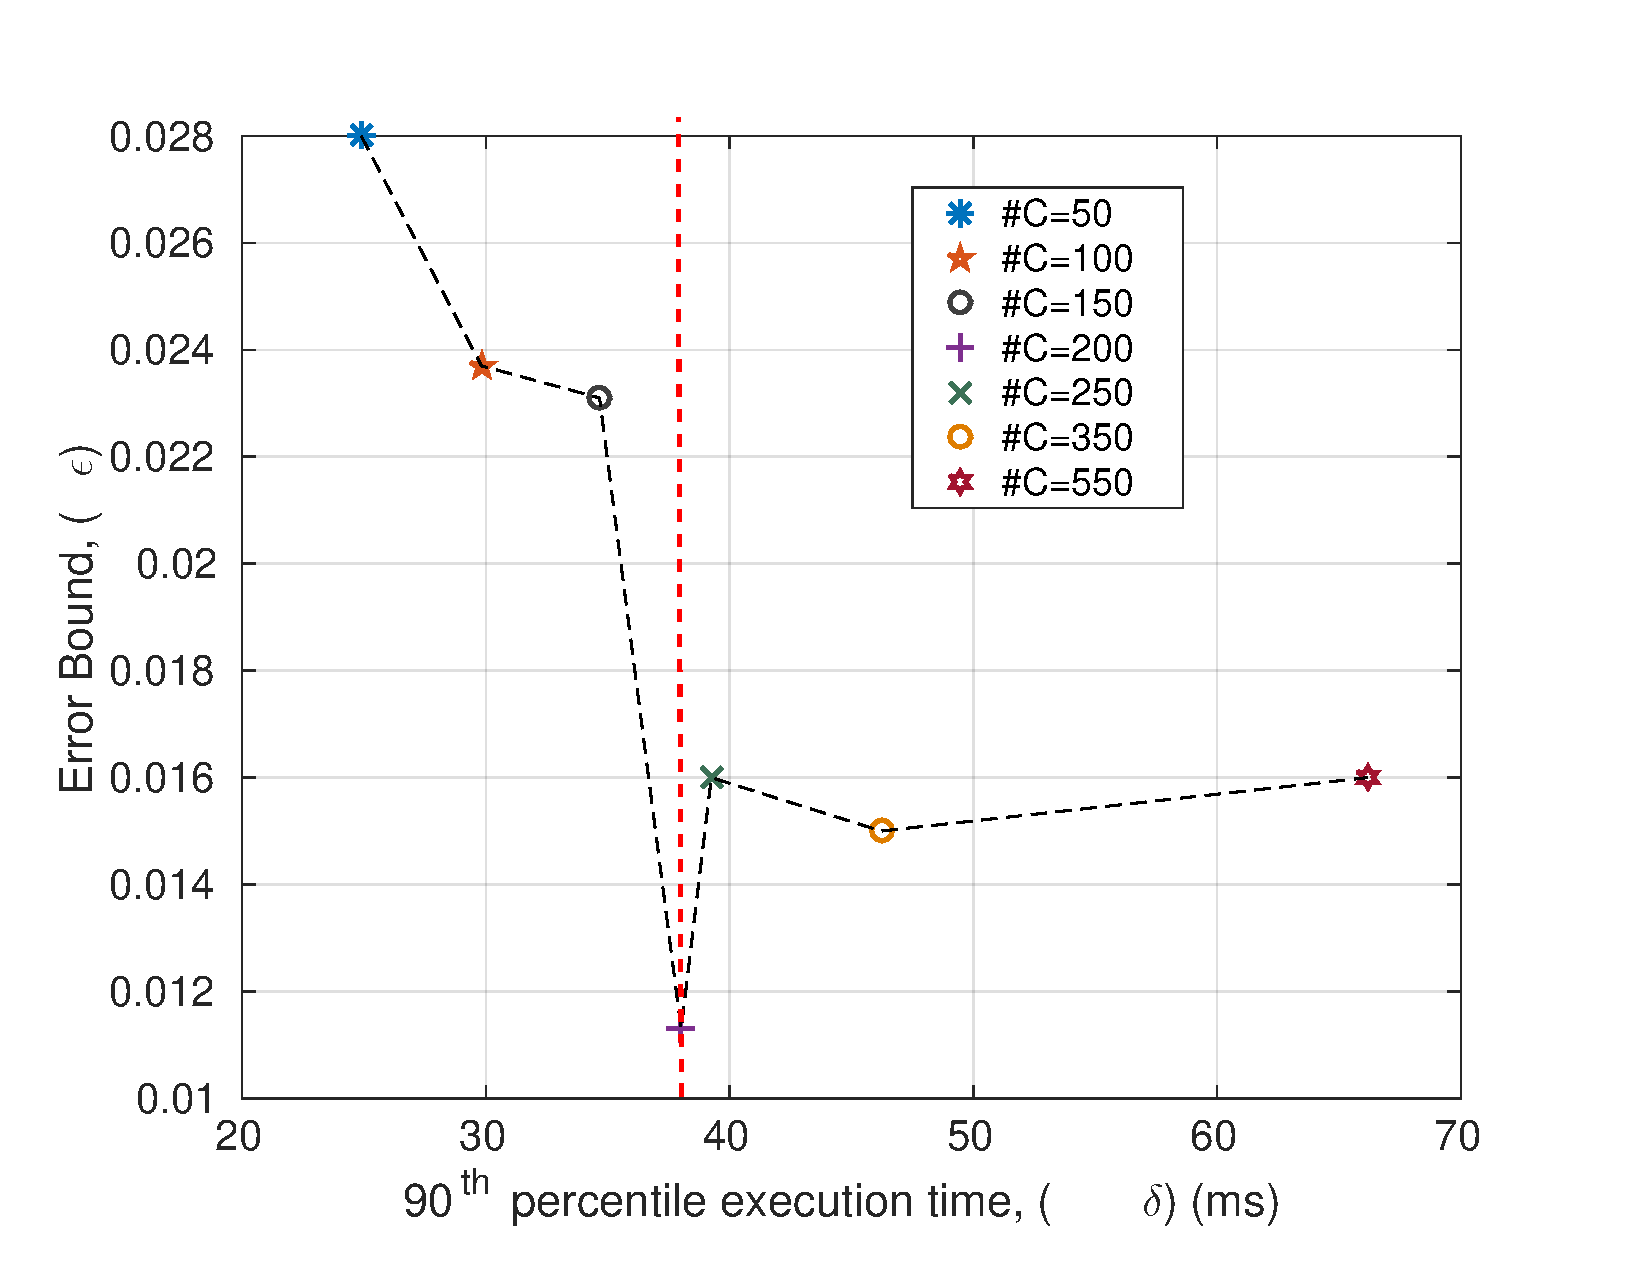
\includegraphics[width=0.9\columnwidth]{figures/errVsTime}
\caption{Error-delay curve for the SVO algorithm running on the Odroid-U3 - ?? Label where we stop choosing delays}
\label{fig:svo_error_delay}
\end{figure}

Fig.~\ref{fig:svoErrVsPower} shows the power consumption vs estimation error, which correlates well with Fig.~\ref{fig:svo_error_delay}.
\begin{figure}[t]
	\centering
	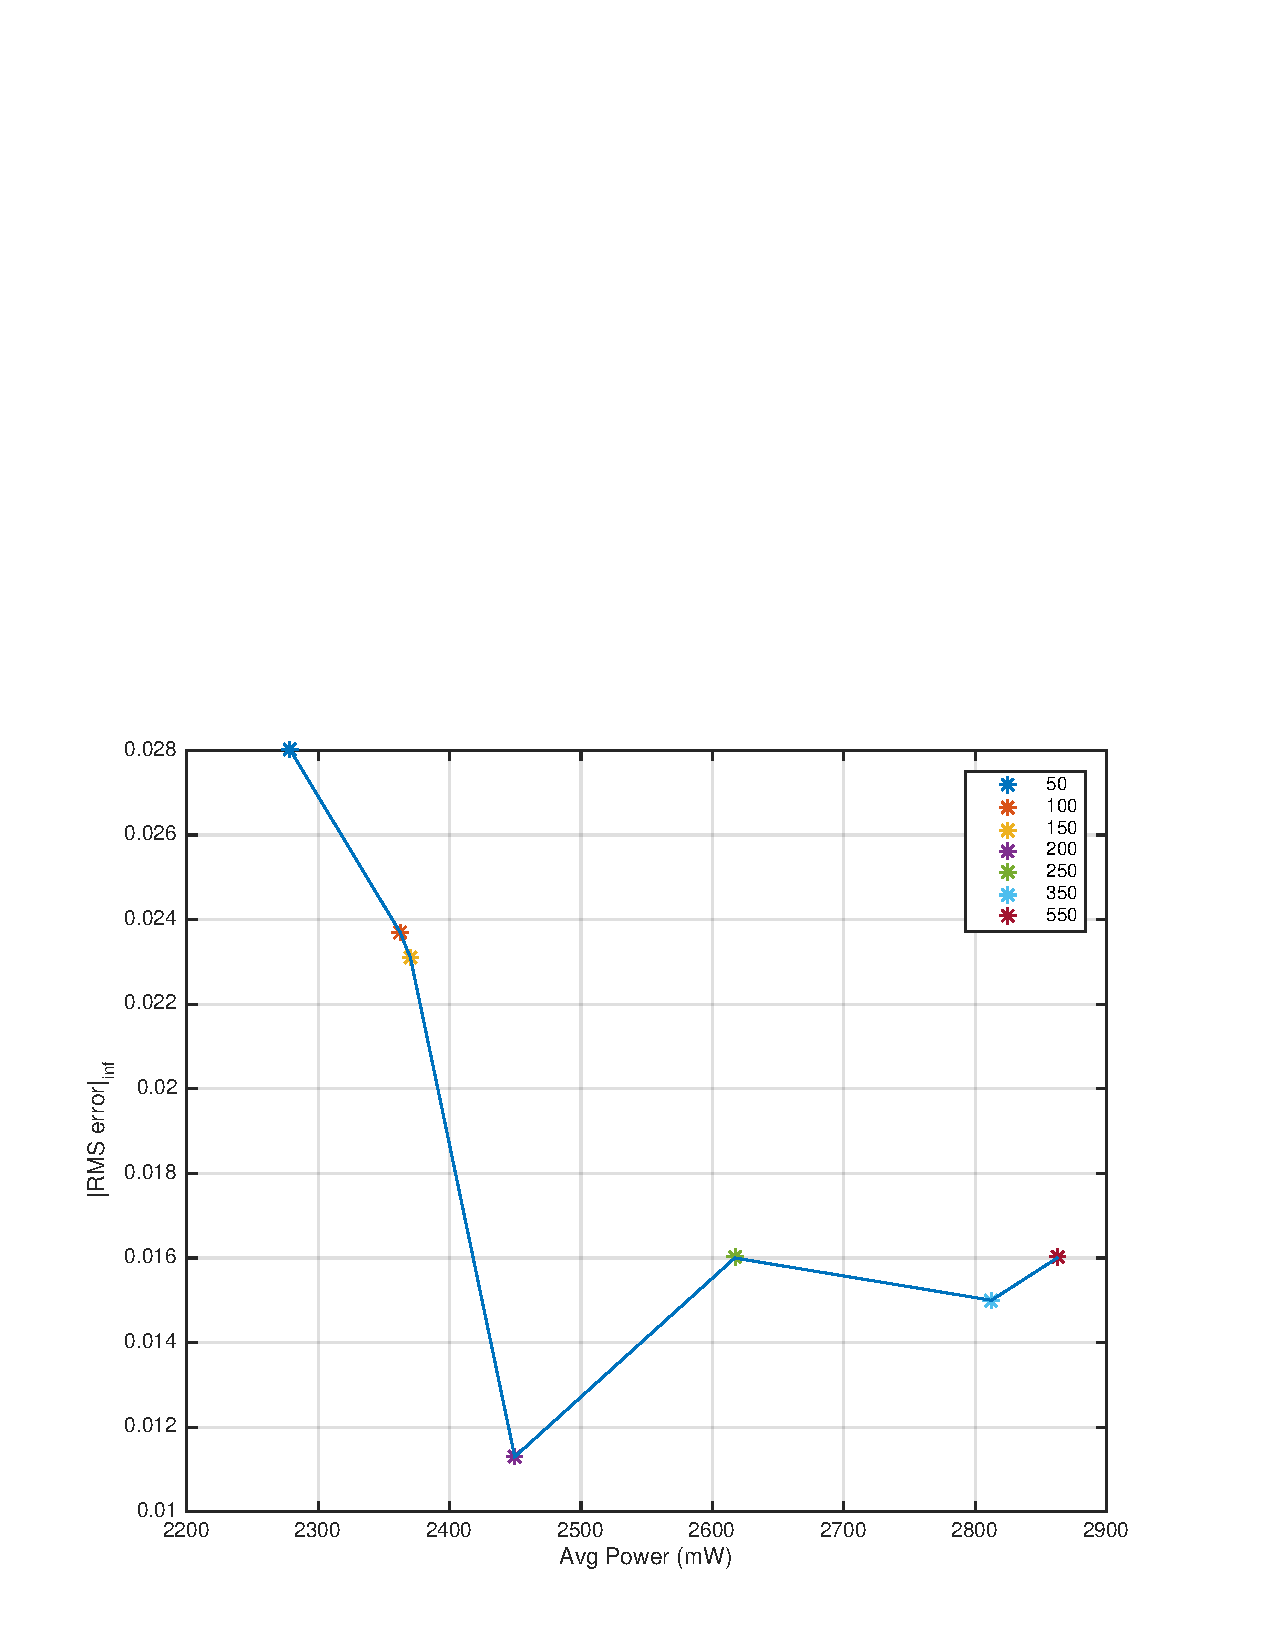
\includegraphics[width=0.9\columnwidth]{figures/errVsPower}
	\caption{Error vs power curve for the SVO algorithm running on the Odroid U3}
	\label{fig:svoErrVsPower}
\end{figure}
